\subsection{Esercizio 19}
Costruire una function Matlab che, specificato in ingresso il grado $n$ del polinomio
interpolante, e gli estremi dell'intervallo $[a, b]$, calcoli le corrispondenti ascisse di Chebyshev.
\newline \textbf{Soluzione:}
% 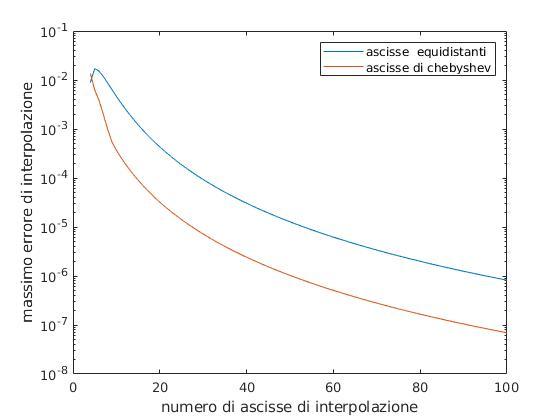
\includegraphics[scale=0.6]{./capitolo4/es19.jpg}\\
% Si nota dai due grafici che la funzione spline riesce a mantenere su entrambe le tipologie di scelta delle ascissi, un basso errore di interpolazione, mentre la funzione splinenat, arriva ad avere nelle ascisse di chebyshev, un andamento simile a quello corrispettivo alla funzione spline, essendo comunque meno preciso. L'uso invece delle ascisse equidistanti nella funzione splinenat, fa si che si abbia un andamento sostanzialmente diverso, rispetto a quello delle corrispettive nella funzione spline, e anche rispetto alle ascisse di chebyshev calcolate dalla stessa funzione.
